% --- Template for thesis / report with tktltiki2 class ---
% 
% last updated 2013/02/15 for tkltiki2 v1.02

\documentclass[english]{tktltiki2}

% tktltiki2 automatically loads babel, so you can simply
% give the language parameter (e.g. finnish, swedish, english, british) as
% a parameter for the class: \documentclass[finnish]{tktltiki2}.
% The information on title and abstract is generated automatically depending on
% the language, see below if you need to change any of these manually.
% 
% Class options:
% - grading                 -- Print labels for grading information on the front page.
% - disablelastpagecounter  -- Disables the automatic generation of page number information
%                              in the abstract. See also \numberofpagesinformation{} command below.
%
% The class also respects the following options of article class:
%   10pt, 11pt, 12pt, final, draft, oneside, twoside,
%   openright, openany, onecolumn, twocolumn, leqno, fleqn
%
% The default font size is 11pt. The paper size used is A4, other sizes are not supported.
%
% rubber: module pdftex

% --- General packages ---

\usepackage[utf8]{inputenc}
\usepackage[T1]{fontenc}
\usepackage{lmodern}
\usepackage{microtype}
\usepackage{amsfonts,amsmath,amssymb,amsthm,booktabs,color,enumitem,graphicx}
\usepackage[pdftex,hidelinks]{hyperref}

% Automatically set the PDF metadata fields
\makeatletter
\AtBeginDocument{\hypersetup{pdftitle = {\@title}, pdfauthor = {\@author}}}
\makeatother

% --- Language-related settings ---
%
% these should be modified according to your language

% babelbib for non-english bibliography using bibtex
\usepackage[fixlanguage]{babelbib}

% add bibliography to the table of contents
\usepackage[nottoc]{tocbibind}

% --- Theorem environment definitions ---

\newtheorem{thm}{Theorem}
\newtheorem{lem}[thm]{Lemma}
\newtheorem{cor}[thm]{Corollary}

\theoremstyle{definition}
\newtheorem{definition}[thm]{Definition}

\theoremstyle{remark}
\newtheorem*{remark}{Remark}


% --- tktltiki2 options ---
%
% The following commands define the information used to generate title and
% abstract pages. The following entries should be always specified:

\title{Distributed Association Rule Discovery from Big Data}
\author{Jiri Hamberg}
\date{\today}
\level{Master's Thesis}
\abstract{Abstract.}

% The following can be used to specify keywords and classification of the paper:

\keywords{keyword 1, keyword 2, keyword 3}

% classification according to ACM Computing Classification System (http://www.acm.org/about/class/)
% This is probably mostly relevant for computer scientists
% uncomment the following; contents of \classification will be printed under the abstract with a title
% "ACM Computing Classification System (CCS):"
% \classification{}

% If the automatic page number counting is not working as desired in your case,
% uncomment the following to manually set the number of pages displayed in the abstract page:
%
% \numberofpagesinformation{16 pages + 10 appendix pages}
%
% If you are not a computer scientist, you will want to uncomment the following by hand and specify
% your department, faculty and subject by hand:
%
% \faculty{Faculty of Science}
% \department{Department of Computer Science}
% \subject{Computer Science}
%
% If you are not from the University of Helsinki, then you will most likely want to set these also:
%
% \university{University of Helsinki}
% \universitylong{HELSINGIN YLIOPISTO --- HELSINGFORS UNIVERSITET --- UNIVERSITY OF HELSINKI} % displayed on the top of the abstract page
% \city{Helsinki}
%


\begin{document}

% --- Front matter ---

\frontmatter      % roman page numbering for front matter

\maketitle        % title page
\makeabstract     % abstract page

\tableofcontents  % table of contents

% --- Main matter ---

\mainmatter       % clear page, start arabic page numbering


\section{Introduction}

\textit{Big Data} is a term coined to capture the essence of large datasets typical for the digital age. Big Data can be described by three aspects: \textit{volume}, \textit{velocity} and \textit{variety}, that make such data difficult to process and analyse by traditional tools and methods~\cite{doi:10.1108/LR-06-2015-0061}. Big \textit{volume} means that the data is simply too large to be processed by traditional tools. Big \textit{velocity} means that the data is growing so quickly that traditional tools cannot keep up with the pace. Big \textit{variety} can refer to high dimensionality or loosely constrained structure of a dataset.

Association rule discovery is an established data mining technique that is commonly used to discover interesting relations from a dataset without making assumptions about its structure. This thesis work explores the applicability of association rule discovery on Big Data. As a practical application of the theory, this thesis will demonstrate how the association rule discovery can be applied to discover relations between mobile device system settings and level of energy consumption from the data produced by Carat~\cite{Oliner:2013:CCE:2517351.2517354}, a collaborative energy diagnosis project.

The Carat project has collected data from over 800,000 mobile devices worldwide since its initiation in 2012~\cite{7840871}. The Carat data is collected from mobile device users that have installed the Carat mobile application to their device. An analysis server collects data samples sent by the Carat mobile applications whenever the battery level of the device changes. The data samples consist of a list of system settings, a list of currently running applications and the current battery level. The analysis server uses the collaborative measurements to identify energy consumption anomalies from the users' applications as well as to estimate the energy consumption of individual applications~\cite{Oliner:2013:CCE:2517351.2517354}.

So far the Carat dataset has not been published in its entirety to ensure the privacy of the participants. As discussed in~\cite{7840871}, it would be helpful for mobile application developers to be able to access the energy consumption data of the users of their application. As a part of this thesis work, a prototype of a Carat developer web API is implemented. The API provides a search engine for mobile application developers, allowing them to search for associations between specific system settings and energy consumption level of the mobile device.   

Key research questions that this thesis attempts to answer are:

\begin{enumerate}
	\item How can association rules be generated efficiently and scalably from Big Data? The solution should be fast enough to be used in a real-time query API. 
	
	\item How to select interesting and useful association rules from the set of all generated rules? 
	
	\item How does the discretization algorithm of continuous variables of the Carat data affect the generated association rules? 
\end{enumerate}  

%Various distributed computing technologies have emerged to tackle the difficulties of processing Big Data. Notably, there are two paradigms of distributed computing that have become increasingly popular over the last decade, namely grid based   


\section{Association Analysis} \label{association analysis}

Association rule mining is the task of finding associations between \textit{items} in a database of \textit{transactions}. The technique was originally developed in 1993 to identify patterns in consumers grocery purchasing behaviour. Since then however, association analysis has found applications in wide variety of domains.

Let us consider a hypothetical dataset shown in table~\ref{table:raw-data}. The dataset consists of mobile device system settings and energy usage measurements. The dataset has three continuous valued variables:  energyRate, the rate at which the battery is discharging;  CPULevel, the device's CPU usage level and screenBrightness, the brightness of the device's screen. Each of these variables takes floating point values ranging from 0 to 1.
\begin{table}[htb]
    \begin{tabular}{ | l | l | l | }
    \hline
    \textbf{energyRate} & \textbf{CPULevel} & \textbf{screenBrightness} \\ \hline
    0.21 & 0.58 & 0.30 \\ \hline 
    0.80 & 0.46 & 0.61 \\ \hline 
    0.76 & 0.65 & 0.93 \\ \hline 
    0.58 & 0.99 & 0.54 \\ \hline 
    \end{tabular}
	\caption{Hypothetical mobile device measurements inspired by Carat dataset}
	\label{table:raw-data}
\end{table}

Since association rule mining requires each variable of the database to be binary valued, a discretization of the variables must be performed. To discretize a continuously valued variable, we need to replace the continuous variable with multiple binary valued variables, each corresponding to an interval or cluster of values of the continuous variable. The details of discretization are discussed in chapter ???. For now, let us consider a naive discretization strategy, where each continuous variable is split to two binary variables by creating two bins at cut point 0.5. Table~\ref{table:discreteData} demonstrates this idea.

\begin{table}[htb]
    \begin{tabular}{ | l | l | l | l | l | l | }
    \hline
    \textbf{energy=low} & \textbf{energy=high} & \textbf{CPU=low} & \textbf{CPU=high} & \textbf{screen=low} & \textbf{screen=high} \\ \hline
    True & False & False & True & True & False \\ \hline 
    False & True & True & False & False & True \\ \hline 
    False & True & False & True & False & True \\ \hline 
    False & True & False & True & False & True \\ \hline 
    \end{tabular}
	\caption{Hypothetical mobile device measurements after naive discretization}
	\label{table:discreteData}
\end{table}

Since every group of variables that is created by discretization is mutually exclusive, a more concise notation for this dataset can be used, as shown in table~\ref{table:discreteDataConcise}.

\begin{table}[htb]
    \begin{tabular}{ | l | l | l |}
    \hline
	\textbf{energyRate} & \textbf{CPULevel} & \textbf{screenBrightness} \\ \hline
    low & high & low  \\ \hline 
    high & low & high \\ \hline 
    high & high & high \\ \hline 
    high & high & high \\ \hline 
    \end{tabular}
    \caption{Hypothetical mobile device measurements after discretization using concise notation}
    \label{table:discreteDataConcise}
\end{table} 

%As an example, consider a hypothetical database of following transactions denoting individual mobile device system settings, extracted from the Carat data:
 
%\begin{center}
%    \begin{tabular}{ | l | l | }
%    \hline
%    \textbf{Items} \\ \hline
%    cpuLevel=high, energyRate=high \\ \hline 
%    diapers, beer, cookies \\ \hline 
%    diapers, beer, bread \\ \hline 
%    butter, bread, cheese \\ \hline 
%    \end{tabular}
%\end{center} 
 
%The goal of the association analysis is then to produce a list of association rules, given a some measure of interestingness. From the database given above, some algorithm might produce the following association rules: 

Having transformed the raw data to binary variables, the goal of the association analysis is then to produce a list of association rules, given some measure of interestingness. For the database given above, an association rule mining algorithm might find the following association rule 

\[
	\left\{ CPULevel=high, screenBrightness=high \right\} \Rightarrow \left\{ energyRate=high \right\}
\]

This rule implies that high CPU utilization together with high screen brightness associates with high level of battery consumption.

\subsection{Formal Problem Definition}

Let $I = \left\{ x_1, x_2, ..., x_n \right\}$ be a set of binary variables called items. A transaction database $T$ is then a multiset of subsets of $I$, where each element of $T$ denotes a transaction. To give the exact problem of association rule discovery, concepts of support and confidence need to be introduced.

Support of an item set $X$ in database $T$ is defined as the fraction of all transactions in $T$ that contain the item set~\cite{Hipp:2000:AAR:360402.360421}.

\[ supp(X) = \dfrac{ \vert \left\{ X' \in T  \mid X \subseteq X'  \right\}  \vert }{ \vert T \vert  } \]

Confidence of a rule $X \Rightarrow Y$, where $X$ and $Y$ are item sets of $T$, is defined as the fraction of transactions in $T$ containing item set $X$ which also contain $Y$~\cite{Hipp:2000:AAR:360402.360421}.

\[conf( X \Rightarrow Y) = \dfrac{ supp( X \bigcup Y ) }{ supp(X) } \]

The problem of association rule discovery can now be formalized the following way. Given a transaction database $T$, minimum support level $s$, where $ 0 \leq s \leq 1 $ and minimum confidence level $c$, where $ 0 \leq c \leq 1 $, find all rules $X \Rightarrow Y$ where $conf( X \Rightarrow Y ) \geq c$, $supp(X) \geq s$ and $supp(Y) \geq s$~\cite{Hipp:2000:AAR:360402.360421}. 

The association rule discovery problem can be further divided into two distinct sub problems, namely frequent pattern mining problem and rule generation problem. A frequent pattern $P$ of database $T$ is a subset of $I$ such that $supp(P) \geq s$. The frequent pattern mining problem is the task of finding all frequent patterns from a given database. The rule generation problem on the other hand, is the task of generating all association rules with sufficient confidence from the frequent patterns. 

\subsection{Frequent Pattern Mining Using Frequent Pattern Growth}

Frequent pattern growth is an efficient algorithm for the frequent pattern mining problem~\cite{Han:2000:MFP:335191.335372}. The algorithm utilizes a specialized data structure called FP-tree, a kind of prefix tree, to speed up the frequent pattern generation. The FP-tree data structure consists of nodes, each of which have tree fields: item name, item count and node link. The item name tells which item the node represents. The item count signifies the number of transactions containing the item, that can be reached by following the path of nodes in the FP-tree leading to this node. The node link contains a pointer to the next node in the FP-tree with the same node name. An exception to this format is the root node of the FP-tree, which does not have any of these fields, but only has links to child nodes. Algorithm~\ref{Algorithm:FP-tree} shows how to constructs a FP-tree for a transaction database~\cite{Han:2000:MFP:335191.335372}.

\begin{algorithm}[!htbp]
	\SetAlgoLined\DontPrintSemicolon
	\SetKwFunction{buildFPTree}{buildFPTree}\SetKwFunction{insertTree}{insertTree}
	\KwData{A transaction database \textit{DB}, minimum support threshold \textit{s}}
	\KwResult{FP-tree for the database}
	\SetKwProg{myalg}{Algorithm}{}{}
	\myalg{\buildFPTree{}}{
		\nl	\textit{F} $\leftarrow$ Scan \textit{DB} and collect a map of items and their frequencies\;
		\nl \textit{L} $\leftarrow$ Sort keys of \textit{F} in descending order of support filtering out items which have support < \textit{s}\;
		\nl \textit{T} $\leftarrow$ root node of the FP-tree\;
		\nl \For{ transaction \textit{Trans} \textbf{in} \textit{DB} }{ 
			\nl sort \textit{Trans} according to \textit{L} and filter out infrequent items\;
			\nl insertTree(\textit{Trans}, \textit{T})\;
		}
		\nl \KwRet{\textit{T}}\;
	}
	\setcounter{AlgoLine}{0}
	\SetKwProg{myproc}{Procedure}{}{}
  	\myproc{\insertTree{\textit{Trans}, \textit{T}}}{
		\nl \If{\textit{Trans} is empty}{
			\nl \KwRet\;
		} \nl \Else{
			\nl	\textit{N} $\leftarrow$ first item of \textit{Trans}\;
			\nl \textit{tail} $\leftarrow$ tail of \textit{Trans}\;	
			\nl \If{ \textit{T} has a child \textit{h} such that \textit{N}.item-name == \textit{h}.item-name} {
				\nl \textit{h}.count += 1\;
				\nl insertTree(\textit{tail}, \textit{h})
			} \nl \Else {
				\nl \textit{n} $\leftarrow$ create new node with item-name = \textit{p}.item-name and count = 1 and link \textit{T} as its parent\;
				\nl insertTree(\textit{tail}, \textit{n})
			}
		}
	}	
	\caption{Fp-tree construction}
	\label{Algorithm:FP-tree}
\end{algorithm}  

The algorithm consists of two procedures. The entry point for the algorithm is the \textit{buildFPTree}-procedure, which takes no parameters and returns the newly built FP-tree. The sub-program \textit{insertTree} takes a transaction \textit{Trans}, that is sorted by descending item frequency, and an incomplete FP-tree \textit{T} as its parameters. The \textit{insertTree} procedure walks down \textit{T} in a path determined by the items in \textit{Trans}, incrementing the counts of nodes on the path. If there is no existing path to walk down on at any point, the \textit{insertTree} creates a new node with count 1 as a child of the last node that was walked over.

The \textit{buildFPTree} procedure proceeds the following way. In line 1, the transaction database is scanned and the different item names together with their frequencies are collected to variable \textit{F}. In line 2, keys of \textit{F} are sorted in descending order of support and items which have support less than minimum support \textit{s}. The sorted and filtered key-count-pairs are stored in variable \textit{L}. In line 3, the root of node of the FP-tree is created and stored in variable \textit{T}. In line 4, a for loop that iterates over each transaction in the transaction database is entered. The loop yields the transactions in a variable called \textit{Trans}. In line 5, the contents of variable \textit{Trans} are sorted according to the ordering induced by \textit{L} and infrequent items (items which have support that is less than \textit{s}) are filtered out of \textit{Trans}. In line 6, the sub-program \textit{insertTree} is called passing parameters \textit{Trans} and \textit{T}. The for loop entered on line 4 is exited. Finally on line 7, \textit{T}, which now contains the complete FP-tree, is returned.  

The \textit{insertTree} procedure consists of the following steps. In lines 1-3, we check if parameter \textit{Trans} is empty and return if so. In lines 4-5, we store the first item of parameter \textit{Trans} in variable \textit{N} and the rest of the items in variable \textit{tail}. In line 6, we enter an if statement with the conditional "\textit{T} has a child \textit{h} such that \textit{h} has the same item name as \textit{N}". In line 7 we increment the count of \textit{N} by one. In line 8 we call \textit{insertTree} recursively with parameters \textit{tail} and \textit{h}. In line 9, we exit the then-branch of the if statement and enter the else-branch. In line 10, we create a new node with item-name equal to \textit{N}, count equal to 1 and we link \textit{T} as the nodes parent. The newly created node is stored in variable \textit{n}. In line 11 we call \textit{insertTree} recursively with \textit{tail} and \textit{n} as its parameters.

To better illustrate the process of building an FP-tree from a transaction database, let us go through an example that uses a simple made up transaction database. First step of building a FP-tree, is to sort each transaction by decreasing order of frequency of its items in the database. Infrequent items are also filtered out based on the minimum support. Table~\ref{table:fp-growth-example1} shows the example transaction database as well as the frequent items in descending order of frequency. A single traversal over the database is required in order to sort the transactions.

For this example, let us consider a minimum support of 0.3. Since the number of transactions in our database is 6 and $ \frac{1}{6} < 0.3 < \frac{2}{6} $, all items with frequency less than 2 can be filtered out. Thus items i and j are not included in the second column of table~\ref{table:fp-growth-example1}. 

\begin{table}[!htbp]
\begin{center}
    \begin{tabular}{ | l | l | }
    \hline
	\textbf{Items} & \textbf{Frequency Ordered and Filtered Items} \\ \hline
    a, b, c, d, e, h & c, e, h, a, b, d \\ \hline 
    c, d, e, h & c, e, h, d \\ \hline 
    c, e, h & c, e, h \\ \hline 
    a, b, c, e, j & c, e, a, b \\ \hline 
    c, h & c, h \\ \hline
    d, i & d \\ \hline
    \end{tabular}
    \caption{Example transaction database for illustrating FP-tree generation.}
    \label{table:fp-growth-example1}
\end{center}
\end{table} 

To construct the FP-tree we start with a node labelled as "root". We then take the first transaction and walk over its elements in the frequency order. We start from the root node of the FP-tree. Since the roo node has no child nodes, we add a child node labelled with "c" and set its count to 1. We remove the item "c" from the transaction being handled. Then we continue the walk from the node labelled with "c". The procedure is repeated with the remaining items of the transaction, continuing the walk from the node labelled "c". The FP-tree after processing the first transaction is shown in Figure~\ref{figure:fp-growth-example1}.

\begin{figure}[!htbp]
	\centering
	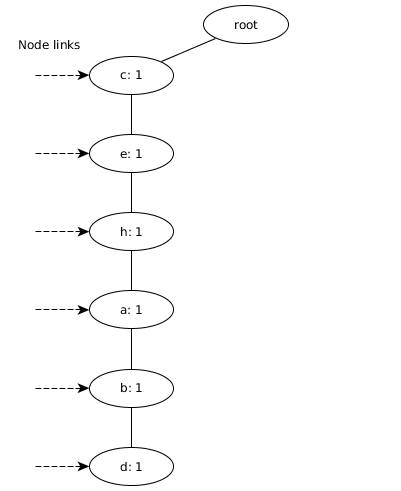
\includegraphics[scale=0.5]{fp-tree-example/fp-tree-p1.png}
	\caption{FP-tree after processing the first transaction}
	\label{figure:fp-growth-example1}
\end{figure}

Next, the second transaction is processed as follows. We again start walking down FP-tree from the root node processing items in the second transaction. Since the root node has a child node labelled with "c" we increment its count to 2 and remove item "c" from the transaction being processed. Since the node has a child node labelled with "e" and our next item to be processed is "e", we move to the node labelled with "e" and increment its count by one and remove item "e" from the transaction being processed. The same process is applied to item "h" and the node labelled with "h". The next item to process is "d", but the node labelled with "h" does not have a child node labelled with "d". We therefore add a child node labelled with "d" and count 1 to the node labelled with "h". Figure~\ref{figure:fp-growth-example2} shows the progress after processing the second transaction of the database.

\begin{figure}[!htbp]
	\centering
	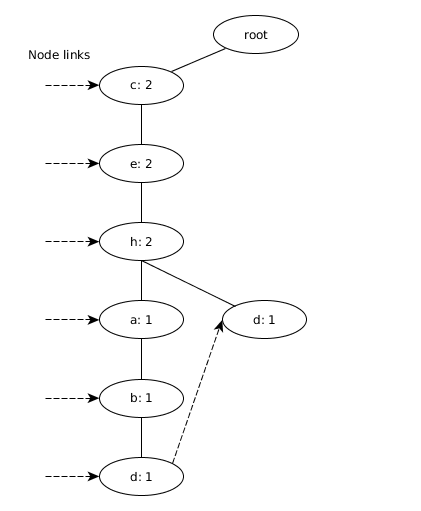
\includegraphics[scale=0.5]{fp-tree-example/fp-tree-p2.png}
	\caption{FP-tree after processing the second transaction}
	\label{figure:fp-growth-example2}
\end{figure}

Repeating the same procedure for the rest of the transactions yields complete FP-tree as illustrated in Figure~\ref{figure:fp-growth-example3}.

\begin{figure}[!htbp]
	\centering
	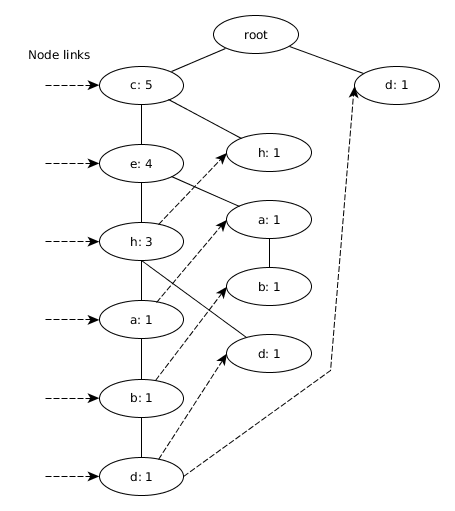
\includegraphics[scale=0.5]{fp-tree-example/fp-tree-p3.png}
	\caption{Complete FP-tree}
	\label{figure:fp-growth-example3}
\end{figure}

The dashed arrows in Figure~\ref{figure:fp-growth-example3} represent node links. The FP-tree maintains a table of linked lists for each distinctly named item. Whenever a node is added to the FP-tree, a pointer to that node is also added to the linked list corresponding to that nodes label.

The way an FP-tree is constructed guarantees, that all FP-trees have the so called \textit{node-link property}~\cite{Hipp:2000:AAR:360402.360421}. What it means, is that for any frequent item, all frequent patterns containing that item can be constructed by following the item's node-links starting from the item's head in the FP-tree header.  


% --- References ---
%
% bibtex is used to generate the bibliography. The babplain style
% will generate numeric references (e.g. [1]) appropriate for theoretical
% computer science. If you need alphanumeric references (e.g [Tur90]), use
%
% \bibliographystyle{babalpha-lf}
%
% instead.

\bibliographystyle{babplain-lf}
\bibliography{references-en}


% --- Appendices ---

% uncomment the following

% \newpage
% \appendix
% 
% \section{Example appendix}

\end{document}